% Project Specifications
\clearpage%if the chapter heading starts close to bottom of the page, force a line break and remove the vertical vspace
\vspace{21.5pt}
\chapter{Implementation}
\section{Software  setup}

First state of project was getting initial programming environment ready, consisting of rp2040 SDK, Arm GCC cross compiler and visual studio code with plugins for debugging and managing the rp2040 CMAKE build process, and a j-link SWD debugger to program and debug on the \gls{mcu} more flexibly than \gls{usb} UF2 flash programming. A logic analyser was also used in initial phases to help monitor the debug traffic for verification of handshake operations till communication was established between boards.

\section{Hardware setup}
%
\begin{figure}[ht]
	\centering
	\AltText{Initial POC hardware setup showing direct soldered wiring between J-Link Edu and a Raspberry pi Pico}{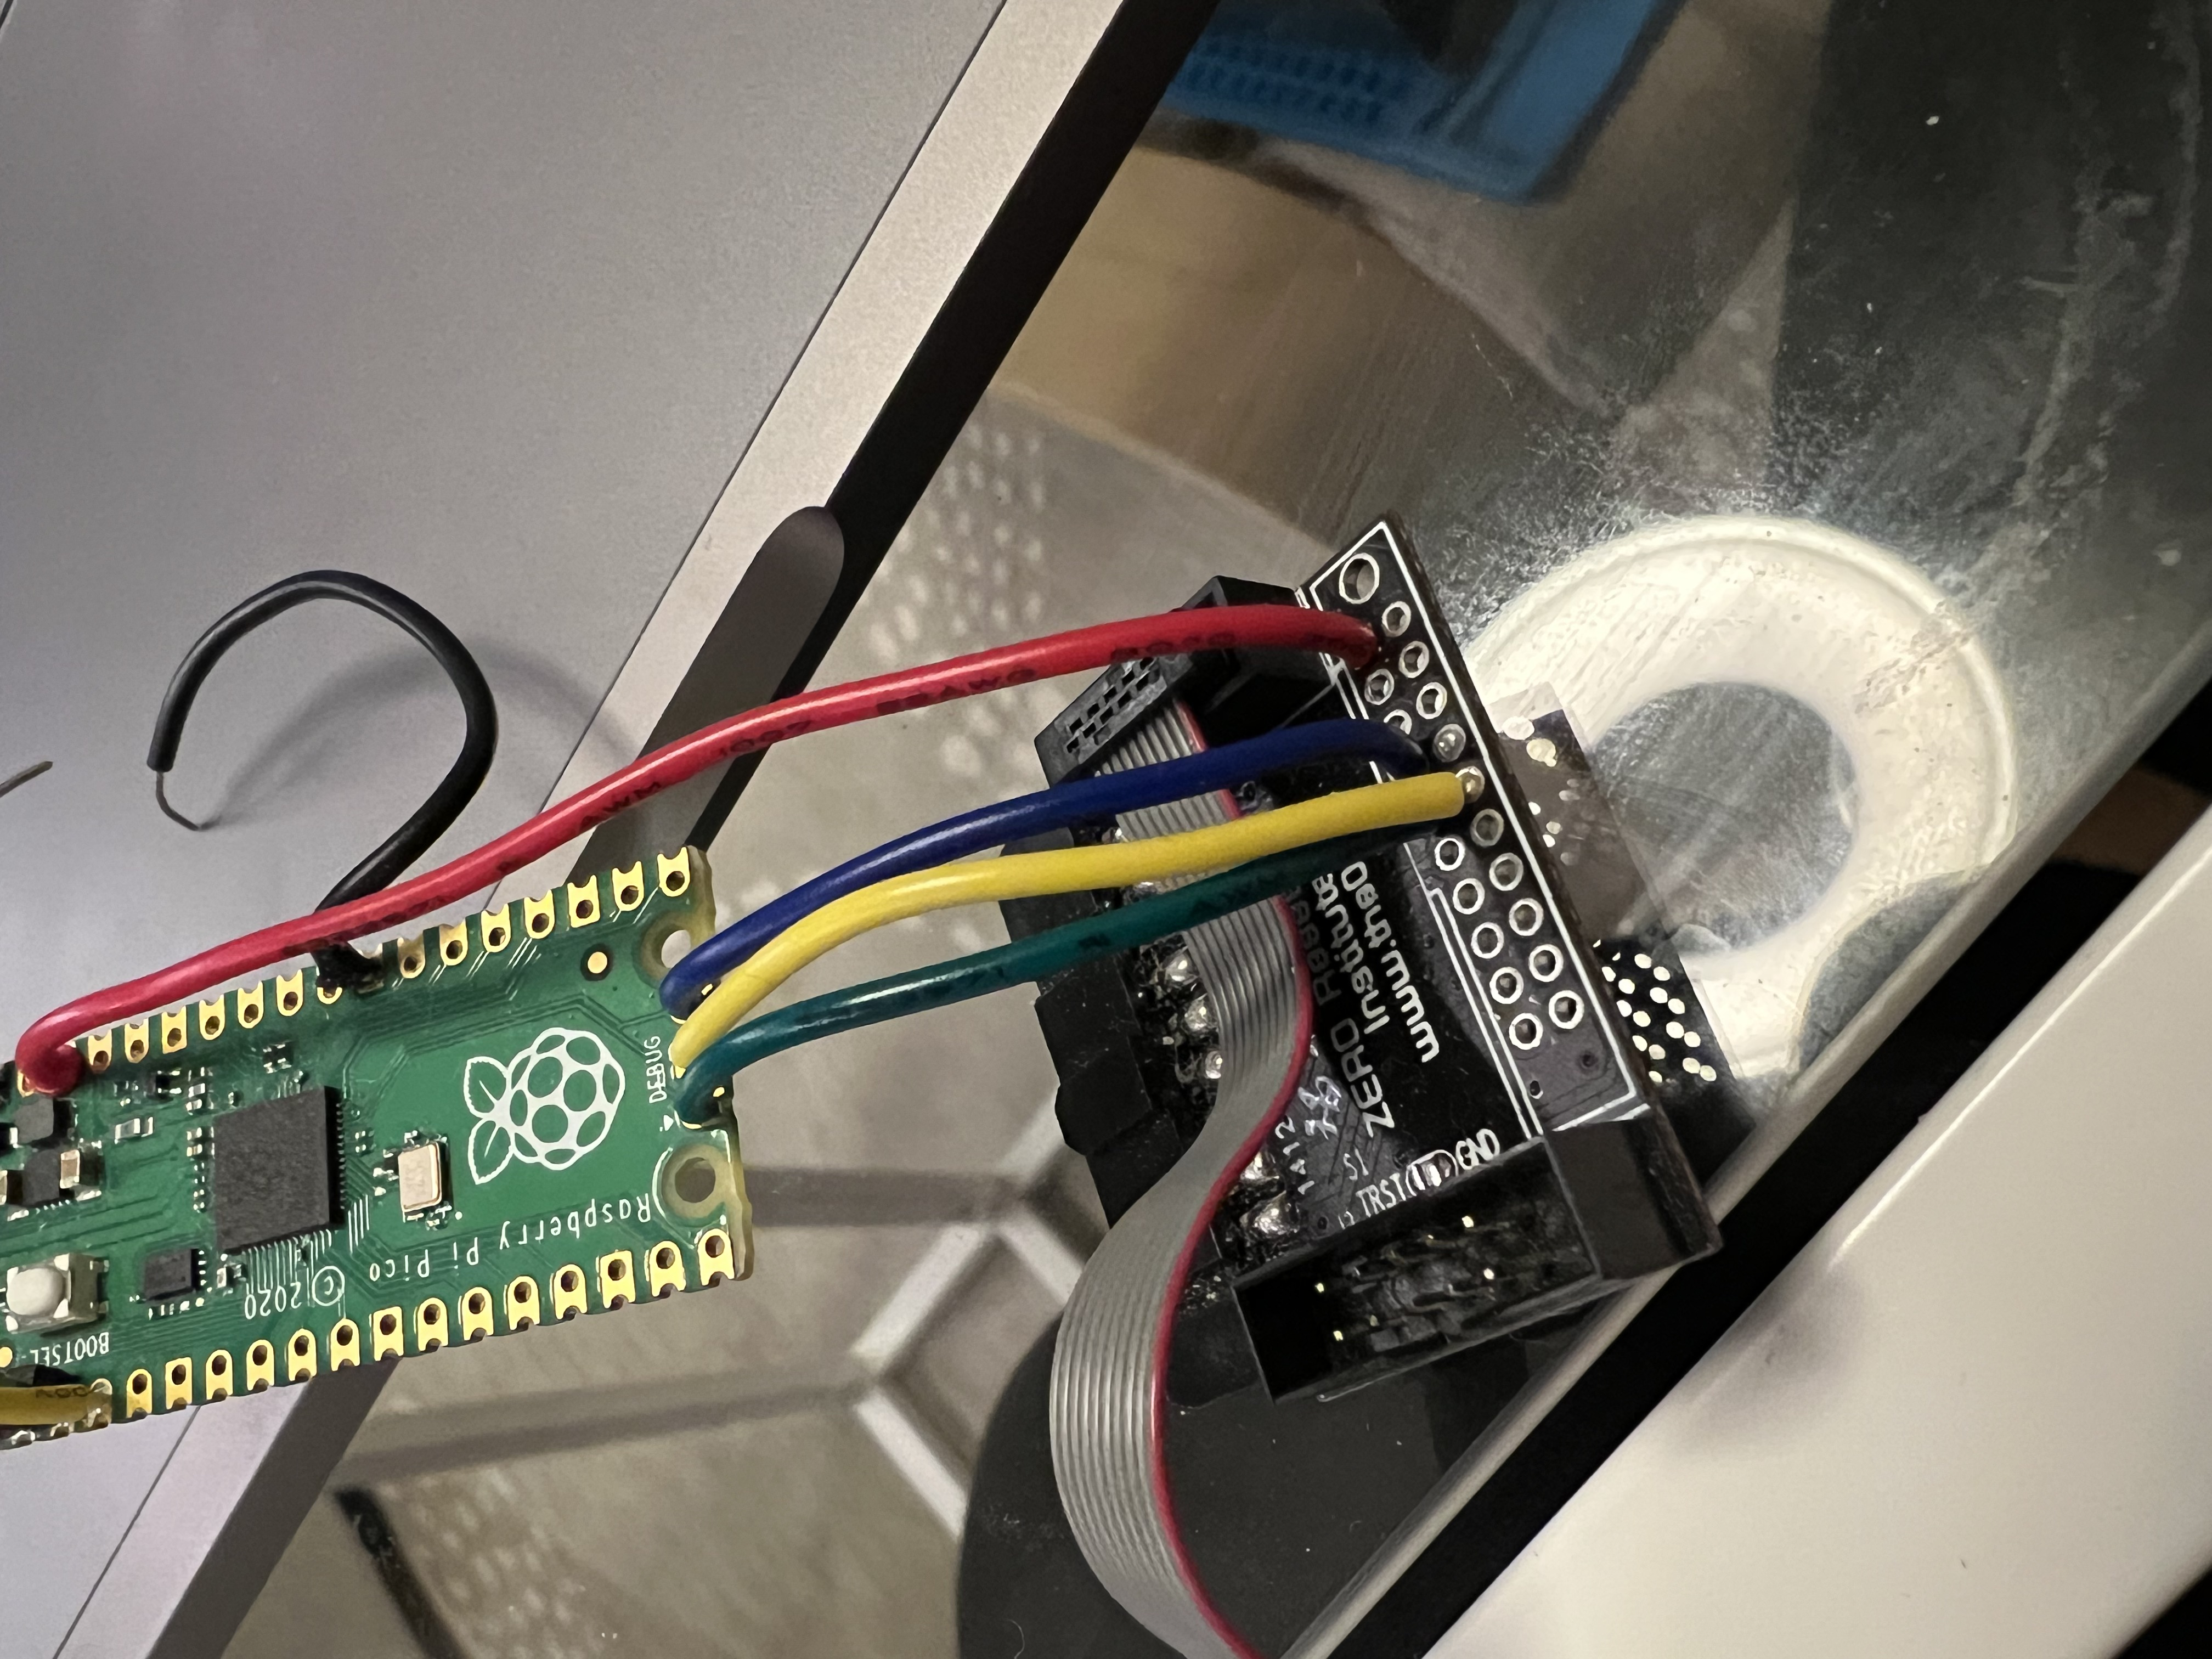
\includegraphics[width=\textwidth]{initial POC setup}}
	\caption{initial POC setup}
	\label{fig:InitialPOCwiring}
\end{figure}

For current proof of concept test bench setup a pair of Pi Pico was directly wired into a J-Link debugger with directly soldered wires for simplicity as show in \autoref{fig:InitialPOCwiring}.

Segger RTT is used for debug console access during testing to eliminate need for a seperate UART/Serial receiver and associated wiring.

In the final test setup a jumper cable is used to simulate the closing of a mounting interface interlock to similate plugging and unplugging target board without physically removing jumper wires from bench setup.

%\pagebreak
\begin{figure}[ht]
	\centering
	\AltText{Full POC hardware setup showing display and buttons for UI on breadboads along with target device}{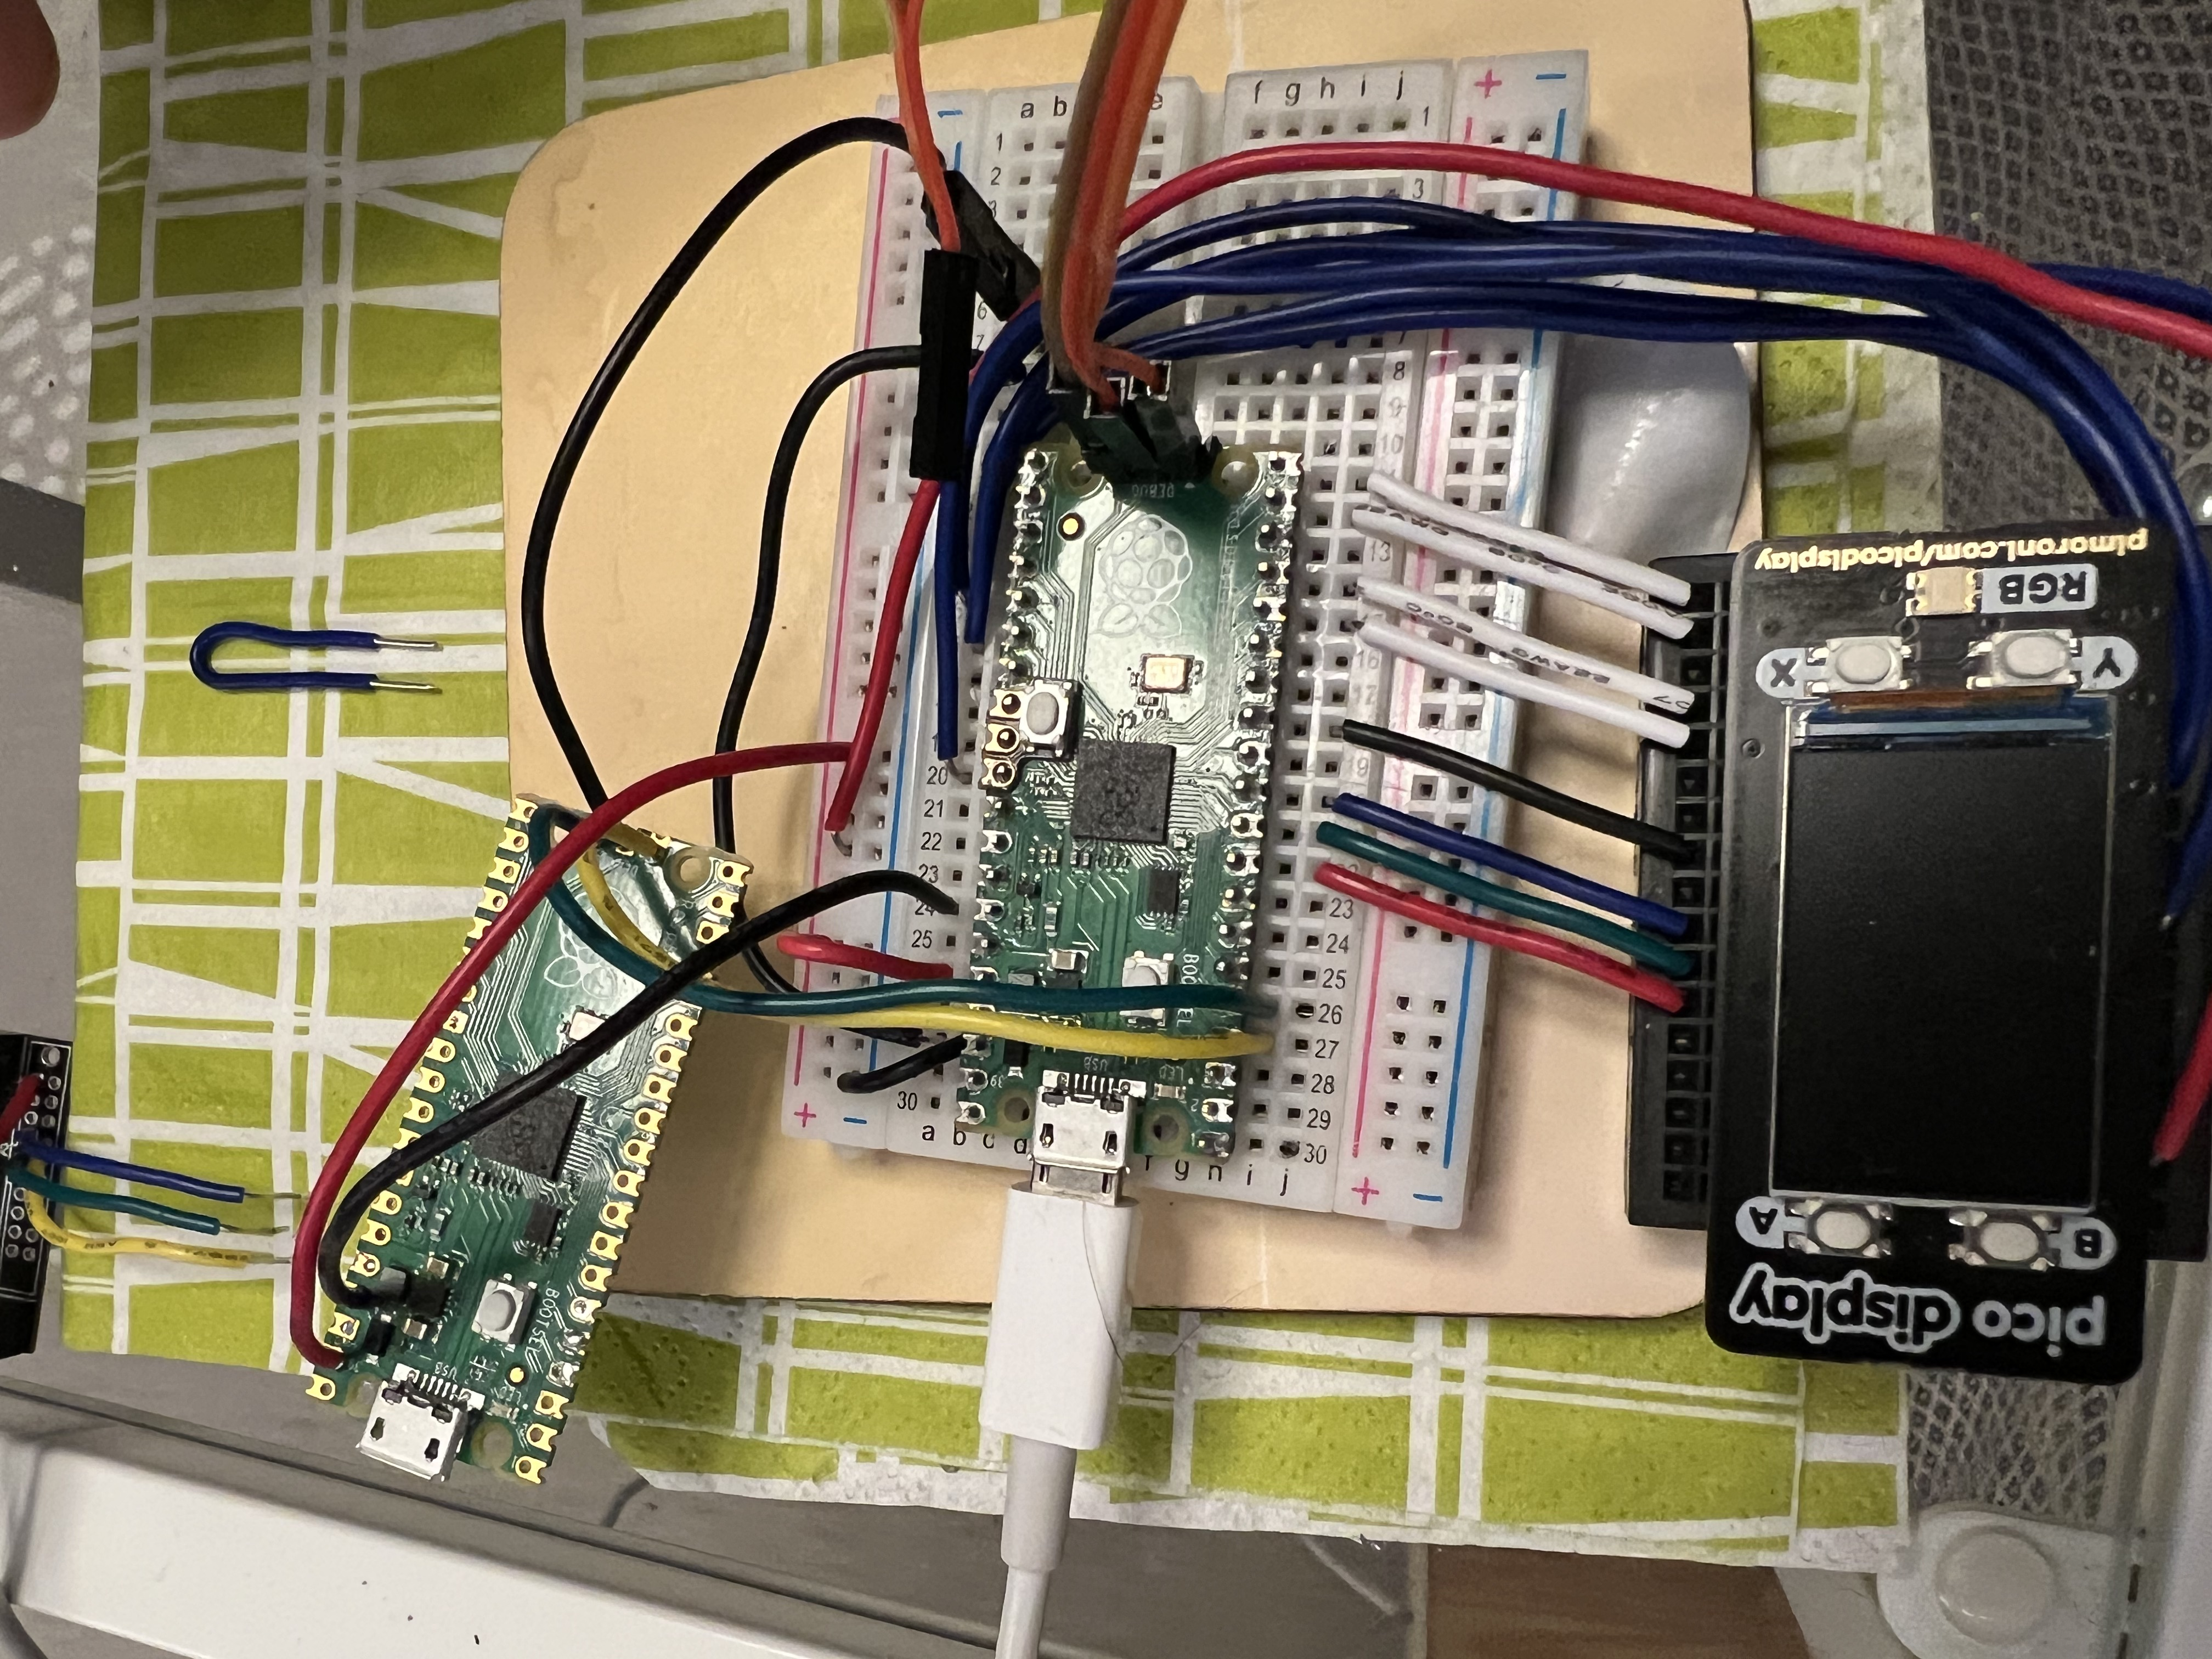
\includegraphics[width=\textwidth]{full POC setup}}
	\caption{Full wiring on breadboard with Interface}
	\label{fig:FullPOCwiring}
\end{figure}

This was later expanded to include a Pimoroni display and buttons for a user interface, and second Pi Pico as flashing target \autoref{fig:FullPOCwiring}.

\section{Software bootstrap}
Initial step was to establish \gls{swd} setup as lowest level critical component, this took longer than anticipated after initial response reading DPIDR succeeded to verify an \gls{arm} debug unit was reponding, but further attempted operations such as memory read failed. Reason for failure transpired to a lack of accounting multiple debug units\cite{raspberrypiltdRaspberryPiPico} with many references to \gls{swd} implementation omitting the step of device selection from the setup sequence owing to most \gls{arm} \gls{mcu}'s only having one core this being an uncessary step.

Once handshake was established the most critical functions of memory write and read were implemented and verified to confirm successful control over \gls{swd}, 

From there a small \gls{ram} resident test program to blink the onboard \gls{led} was created as a test case binary to to be writte and executed from memory via \gls{swd} for a simple control verification, initially merely blinking LED to confirm code execution before building a shared memory structure for executing commands such as file recovery or flash programming/erasing.

This uses magic numbers and checksums for validation, and writing result codes back to memory that can be read by recovery device.

Programming sequence example to bootstrap running code on the target can be found in Appendix 1.


Picture of loading UI

Picture of flashing operation


\section{Testing}

For testing functionality, various likely scenarios were setup and verified repeatably.

First tests consisted of setting up recovery scenarios on MicroPython via Thonny, creating startup python scripts that both block the USB port or just run, and performing a recovery procedure to verify that the file is renamed successfully, or deleted, if a previous recovery result is still present.

Second tests verified that a populated file system could be wiped on an existing MicroPython install.

Third tests verified loading of different uf2 firmware files to the recovery platform, and then reflashing a target pico with the loaded firmware.



